\section{Ground Station Image Viewer (ps)}
\label{sec:ground_station_image_viewer}
The GUI needs a long winded testing. This is because the buttons have to be click and test one by one separately. Because of this, some function of the UAV that does not need a button to test will have its own console application to test it in order to save time. The programmer has to detect most bugs in the real operationThis part is very important because for any program if it caught an error, the program will end unexpectedly.
\subsection{Using Console Application: Testing Connection to UAV, Send Token to Stream Port}
\label{sec:testing_connection_send_to_stream}
The UAV connector use .NET class called System.Net.Sockets. The method that will be using from this class is Sockets.Connect(), Sockets.Send(), Sockets.Receive(). To test the function of this class the programmer develop a separate console application in order to debug only the specific part of the program. Sockets.Connect can be tested by using the Console to display the error code of the running application. The problem could be wrong host name and port number. Therefore, the user are not allowed to change these values. The other problem found in the program is that the programmer forgot to connect the UAV, tell the GCS to enable the enable the network server, and tell the GCS to stream data. Appendix\ref{appen:connectorTest} shows a Connector class that use for testing the Socket connect, read and write method.
Figure \ref{connect to Stream Port} shows a console application testing of the connect function. 
The method is to send a zero token to the data stream and in the GCS program it will display text,\texttt{''\* New datastream client connected from 127.0.0.1:49586''} which it is highlighted in green. 
This text shows that the program works properly and we have accessed to the datastream port of the UAV.
However, the command that send the datastream has not tested in this part. 
This will test the Milestone \ref{sec:ms_basic_dummy_server_comms}.
\begin{figure}[H]
\begin{center}
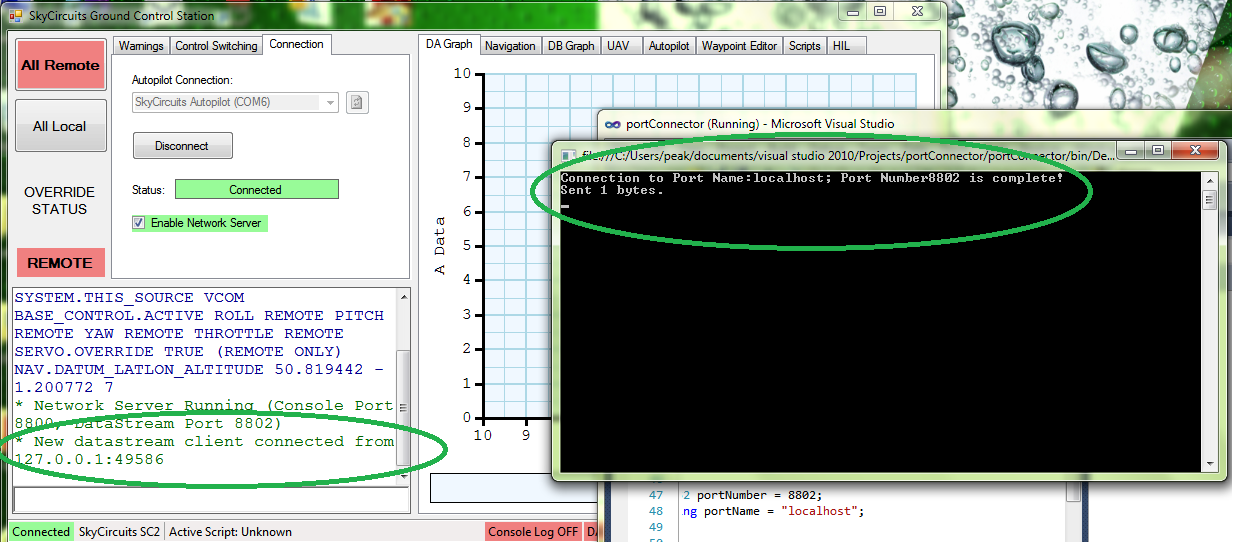
\includegraphics[width=1.00\textwidth]{testing_screenshots/test_sending.png} 
\end{center}
\caption{A screen shot showing the connection with the UAV was successful\label{connect to Stream Port}}
\end{figure}

\subsection{Using Console Application: Testing Connection to UAV, Receive Data from Stream Port}
\label{sec:testing_receive_stream}
Figure\ref{test screenshot} shows a data stream back our testing console application.
Firstly, in the GCS program, we write ''da 30 ht''. 
This code will make the height data stream to the ground station, this data will display on the graph and in the console application, and we can see the number clearly changed when the height has changed.
This is testing that the data stream is working correctly and we have a correct way of getting the data.
Therefore, the Milestone \ref{sec:ms_gs_basestation_comms} is validated.
\begin{figure}[H]
\begin{center}
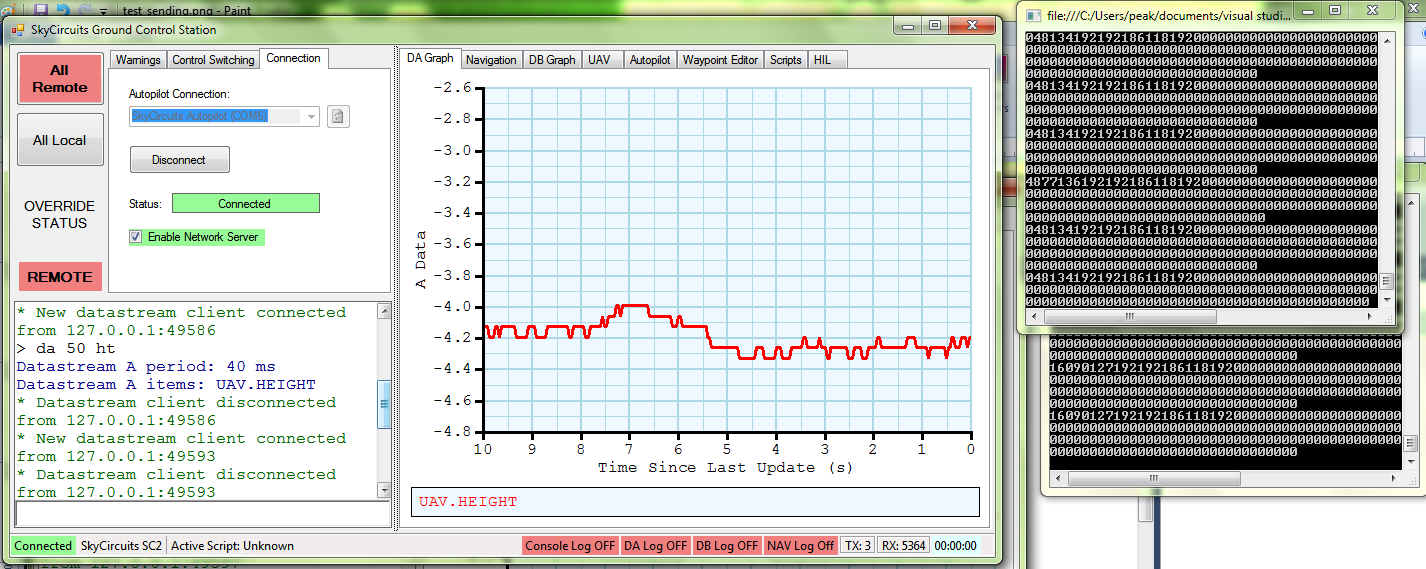
\includegraphics[width=1.00\textwidth]{testing_screenshots/test_data.png} 
\end{center}
\caption{A screen shot shows that the data stream successfully\label{test screenshot}}
\end{figure}

\subsection{Using Console Application: Testing Send Command to Console Port}
\label{sec:send_console}
Figure\ref{test text} show a communication with the console port.
The ground station program allow the programmer to use the console port to send a string command to it. 
This string command can be test that it is correct by the ground station program will produce a line with ''@'' sign on the front of the command sent from the outside of the program.
If the data is correct, the ground station program will detect it and send the data to UAV. 
In the console program, when the user type anything in the console line, it will send byte data to the GCS program.
If the text is a command, the program will process the command and send a byte value as set in the command to the UAV.
The first test is try type 'hi' into the console line.
The GCS will then see the word 'hi' but there is no command available for it.
Therefore, in the GCS console line, it display 'unknown class HELLO'.
Because we send the word via the console line, there is a \@ sign in front of the 'hello' word in GCS program.
The next line we type in is ''da 50 b''.
GCS program know this command therefore it changes the display in the graph to give information about banking of the UAV.
This test validates Milestone\ref{sec:ms_basic_dummy_server_comms}.
\begin{figure}[H]
\begin{center}
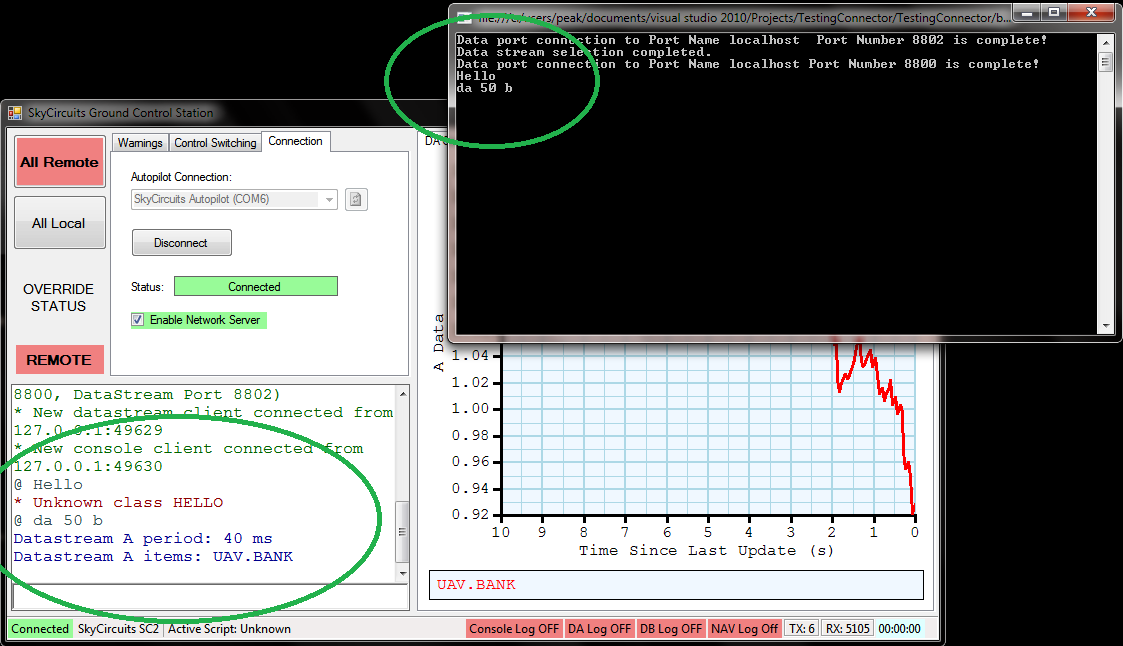
\includegraphics[width=1.00\textwidth]{testing_screenshots/test_sending_test_text_useful.png} 
\end{center}
\caption{A screen shot showing the text sending change the GCS (Ground Control Station) graph value\label{test text}}
\end{figure}

\subsection{Using Window Application: Testing Get Image Button}
\label{sec:test_get_image_button}
The connection between the aircraft and the ground station is using TCP port, it allows the data to send from the aircraft in any form of data. 
In order to test this relationship, a camera will take a picture that the developer know what the picture look like. 
If the picture display an image the same as we expected, the image data is correct.
Figure\ref{camera testing1} shows completed, combined classes together and receive image data.
This testing combined all the existing method together in the Window application.
At this point the connector class will be in the main window application.
When the user click on 'Get Picture' button on the window application, the program will communicate bidirectional, send and receiving which already stated in section\ref{get image algorithm}. 
From the figure, it clearly see that the image is downloading and the image has displayed correctly. This test validates Milestone \ref{sec:ms_gs_recieve_image}. 
\begin{figure}[H]
\begin{center}
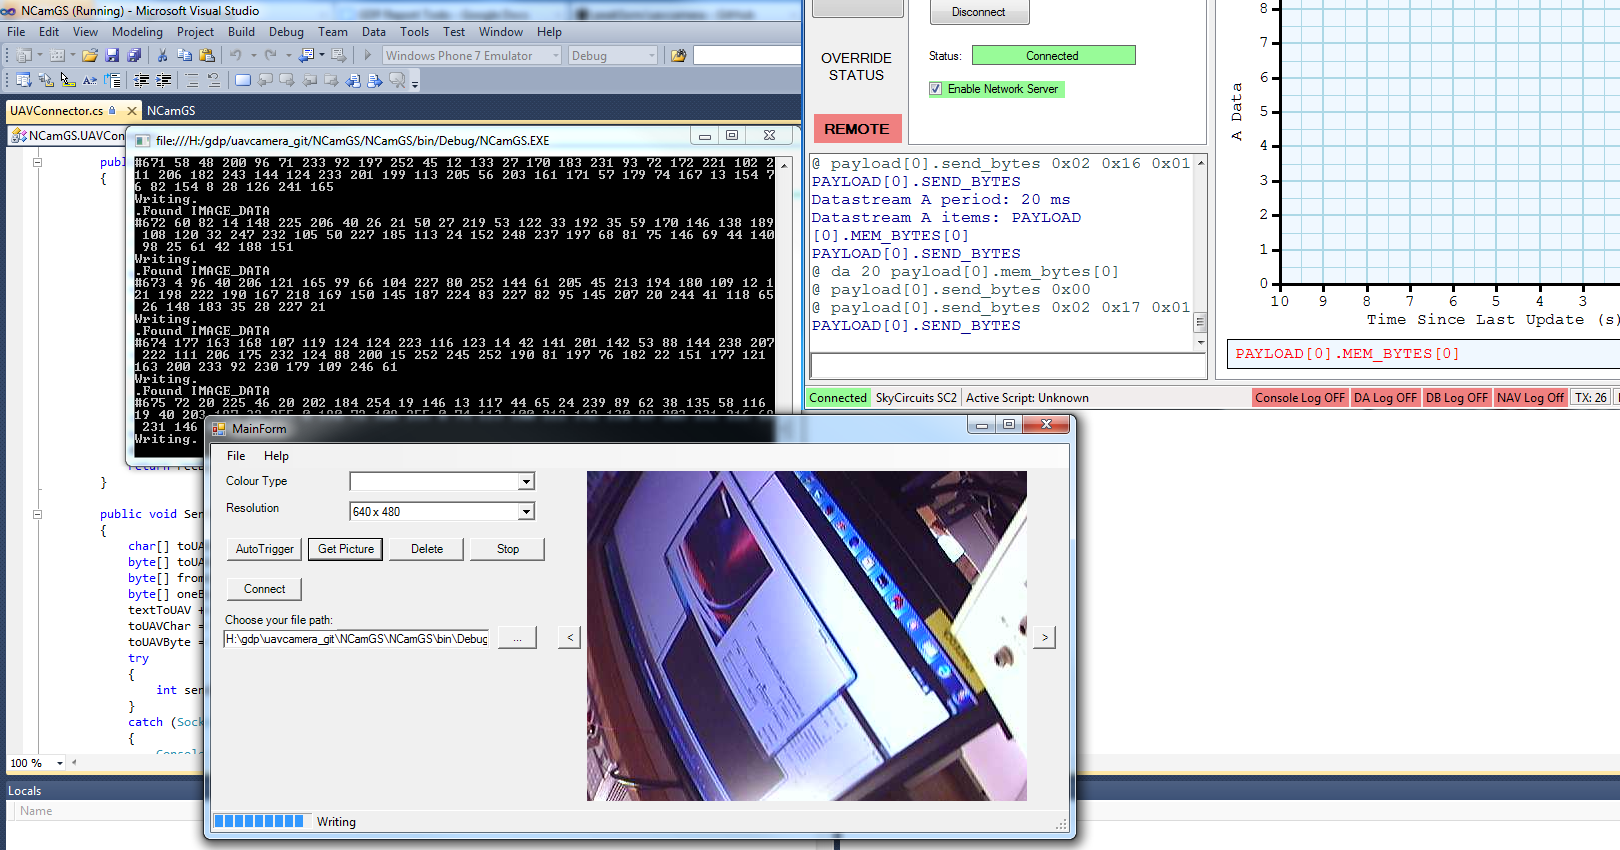
\includegraphics[width=1.00\textwidth]{testing_screenshots/cam_test_11.png} 
\end{center}
\caption{A screen shot showing the picture has been taken correctly\label {camera testing1}}
\end{figure}

\subsection{Using Window Application: Testing Resolution Option}
\label{test_res_op}
When the resolution option changes, the Image viewer program will change the command byte that send to the Console Port of the UAV. 
This can be test by changing the combo box in the image viewer program and click on the Get Picture button.
If it is working correctly, the ground station will see the correct resolution chosen of the picture taken.
Figure \ref{resolution testing} shows a working resolution changing module. 
The putty shows the resolution command that sent back from the payload.
Therefore, it has proved that the resolution option is working.
This test complete the Milestone \ref{sec:ms_pl_img_gs_cam_res}.
\begin{figure}[H]
\begin{center}
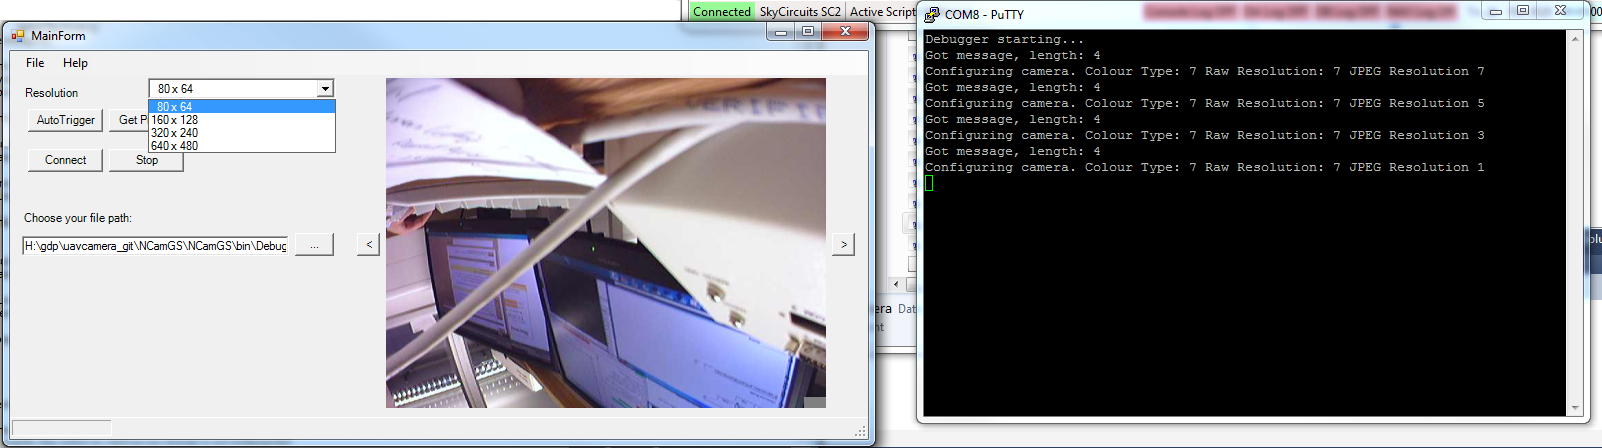
\includegraphics[width=1.00\textwidth]{testing_screenshots/change_res_ncam_1.png} 
\end{center}
\caption{A screen shot showing that the resolution chosen send different signal to the payload\label{resolution testing}}
\end{figure}

\subsection{Functional User Interface}
\label{func_UI}
The tests listed above verifying Milestone \ref{sec:ms_gs_func_interface} is completed. The figure\ref{completeGUI} shows a complete user interface that is functional and ready for the customer to use.
\begin{figure}[H]
\begin{center}
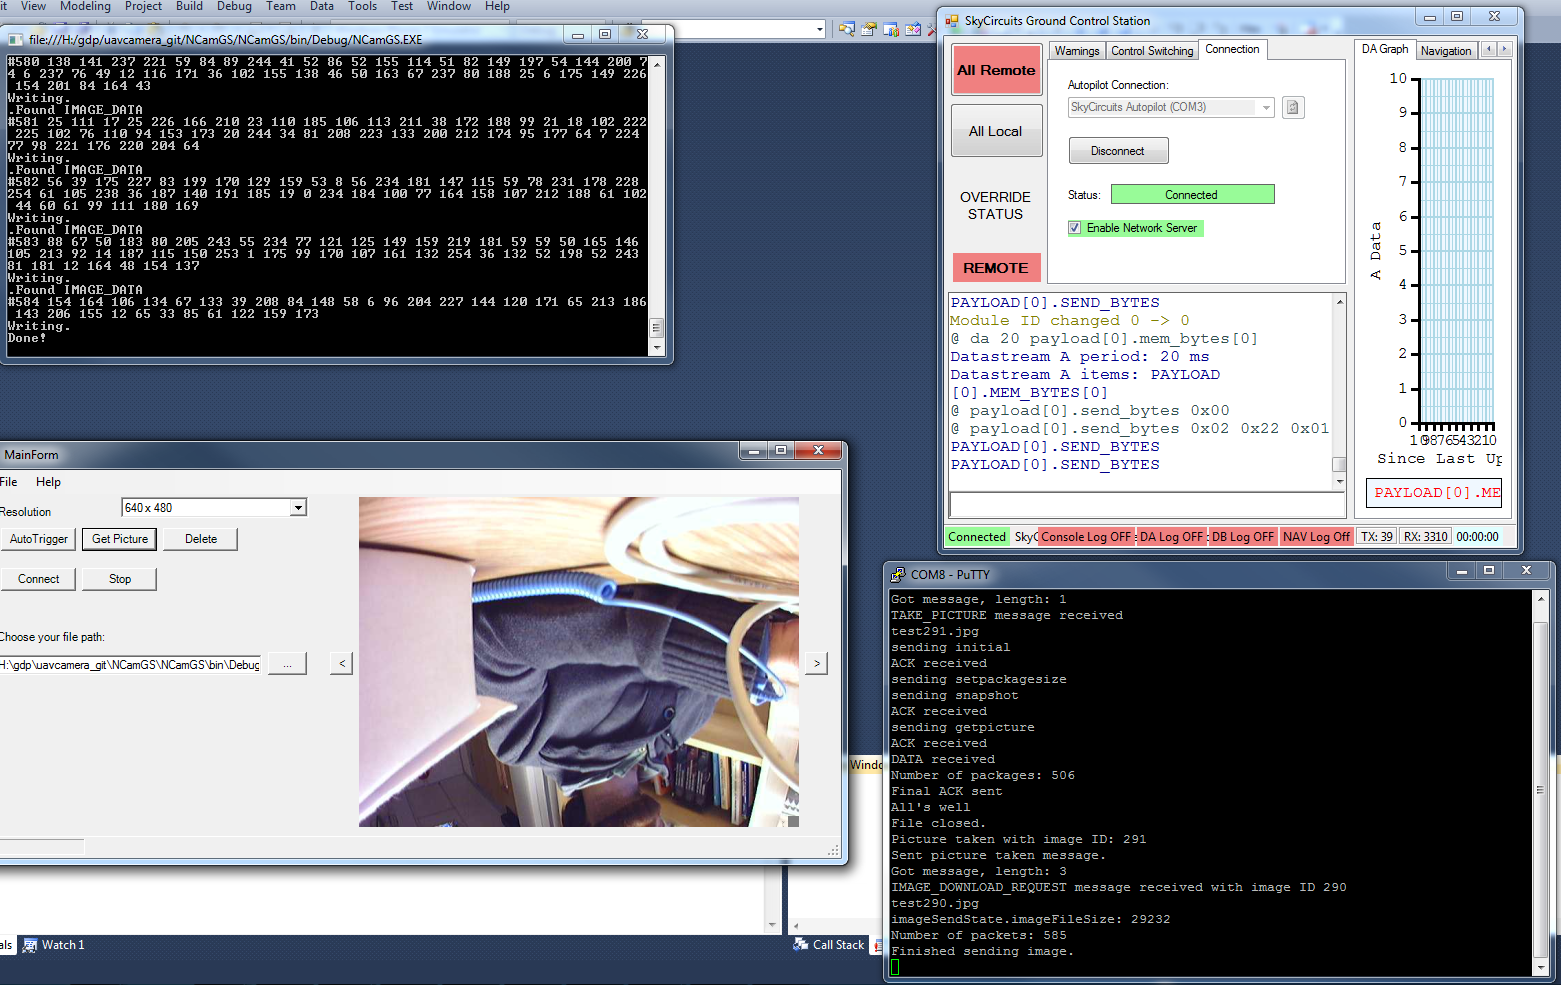
\includegraphics[width=1.00\textwidth]{testing_screenshots/complete_testing_3.png} 
\end{center}
\caption{A screen shot showing a complete UI\label{completeGUI}}
\end{figure}



